
	\begin{subfigure}{0.45\textwidth}
		\centering
		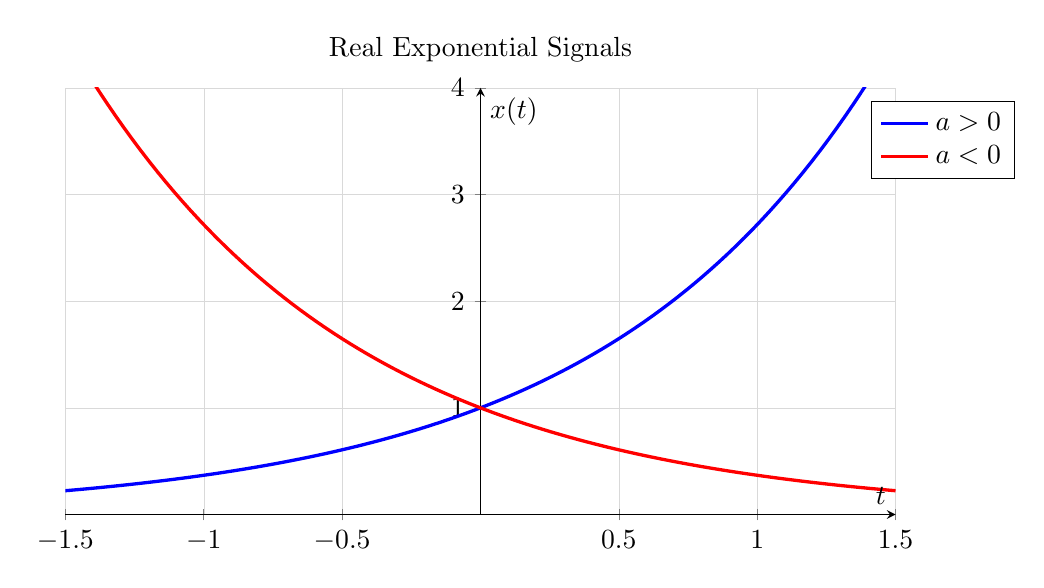
\begin{tikzpicture}
			\begin{axis}[
				width=\linewidth,
				height=7cm,
				title={Real Exponential Signals},
				xlabel={$t$},
				ylabel={$x(t)$},
				axis lines=middle,
				xmin=-1.5, xmax=1.5,
				ymin=0, ymax=4,
				ytick={1,2,3,4},
				grid=major,
				grid style={line width=.1pt, draw=gray!30},
				legend style={
					at={(0.97, 0.97)},
					anchor=north west,
					legend cell align={left}
				},
				no marks,
				]
				\addplot[blue, very thick, domain=-1.5:1.5, samples=100] {exp(x)};
				\addlegendentry{$a>0$}
				
				\addplot[red, very thick, domain=-1.5:1.5, samples=100] {exp(-x)};
				\addlegendentry{$a<0$}
			\end{axis}
		\end{tikzpicture}
		\caption{Real exponential signals.}
		\label{fig:real_exp}
	\end{subfigure}
	\hfill
	% --- Second Subfigure: Complex Exponential ---
	\begin{subfigure}{0.5\textwidth}
		\centering
		\begin{tikzpicture}
			\begin{axis}[
				width=\linewidth,
				height=8cm,
				title={Complex Exponential $e^{j\omega_0 t}$},
				xlabel={$\text{Re}$},
				ylabel={$\text{Im}$},
				axis equal image,
				axis lines=middle,
				xmin=-1.5, xmax=1.5,
				ymin=-1.5, ymax=1.5,
				xtick={-1,1},
				ytick={-1,1},
				grid=major,
				grid style={line width=.1pt, draw=gray!30},
				]
				% Draw the unit circle
				\addplot[black, dashed, domain=0:360, samples=361, no marks] ({cos(x)}, {sin(x)});
				
				% Define the angle and coordinates for the vector
				\pgfmathsetmacro{\myangle}{40}
				\coordinate (O) at (axis cs:0,0);
				\coordinate (P) at (axis cs:{cos(\myangle)},{sin(\myangle)});
				\coordinate (X) at (axis cs:1,0);
				
				% Draw the phasor (vector)
				\draw[-stealth, blue, very thick] (O) -- (P) node[above right, black] {$e^{j\omega_0 t}$};
				
				% Draw and label the angle
				\pic [draw, ->, "$\omega_0 t$", angle eccentricity=1.5, font=\small] {angle = X--O--P};
				
				% Label the magnitude
				\node[anchor=north east, font=\small] at (axis cs:1.4, -1.1) {$|e^{j\omega_0 t}|=1$};
			\end{axis}
		\end{tikzpicture}
		\caption{Complex exponential signal.}
		\label{fig:complex_exp}
	\end{subfigure}
	\label{fig:exp_signals}